% % Permutation 2
% middle2(X, [First|Xs]) :-
% append1(Middle, [Last], Xs),
% middle2(X, Middle).
% middle2(X, [X]).

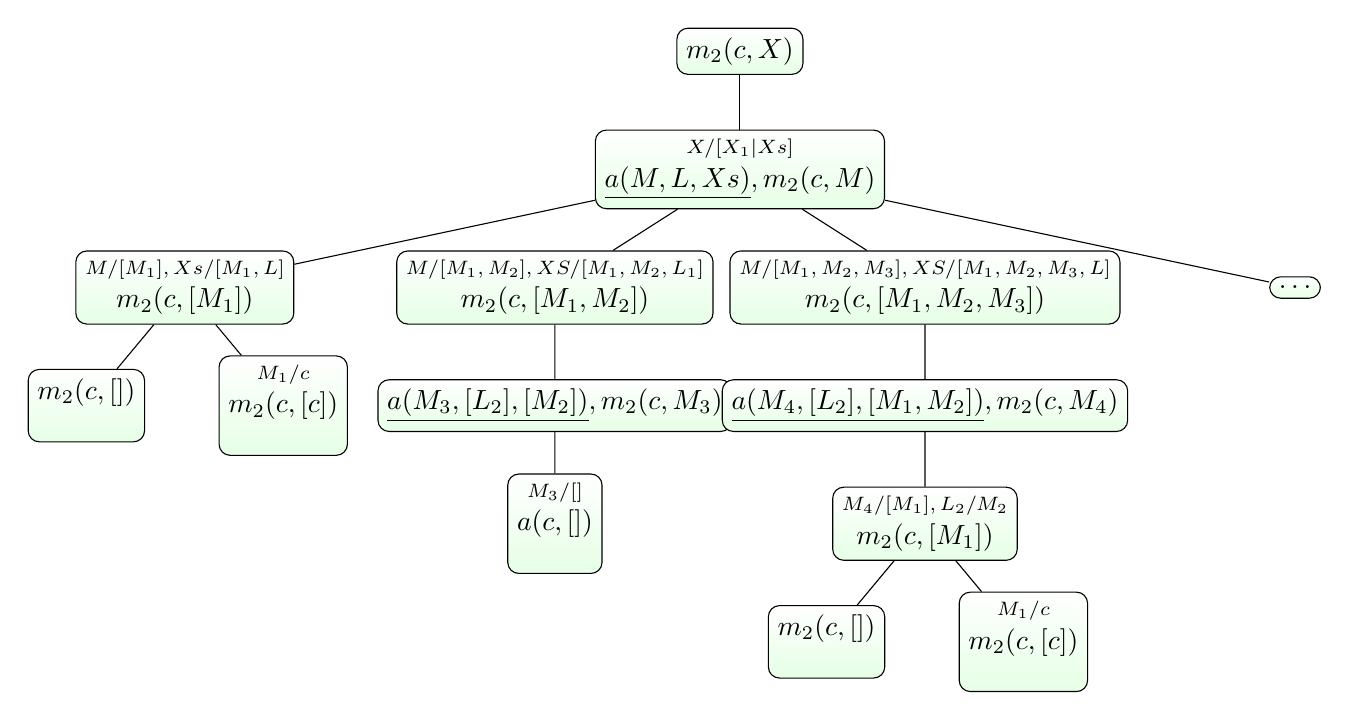
\begin{tikzpicture}[sibling distance=12em, align=center,
  every node/.style = {shape=rectangle, rounded corners,
    draw, align=center,
    top color=white, bottom color=green!10},
    level 1/.style={sibling distance=4cm},
    level 2/.style={sibling distance=4.7cm}, 
    level 3/.style={sibling distance=2.5cm}, ]
  \node {$m_2(c,X)$}
    child { node {\scriptsize $X/[X_1|Xs]$\\$\underline{a(M,L,Xs)},m_2(c,M)$}
      child { node {\scriptsize $M/[M_1], Xs/[M_1,L]$\\$m_2(c, [M_1])$}
        child { node { $m_2(c,[])$\\ $\square$}}
        child { node { \scriptsize $M_1/c$\\ $m_2(c, [c])$\\$\blacksquare$}}
      }
      child { node {\scriptsize $M/[M_1,M_2], XS/[M_1,M_2,L_1]$\\$m_2(c,[M_1,M_2])$}
        child { node {$\underline{a(M_3, [L_2], [M_2])},m_2(c, M_3)$}
          child { node {\scriptsize$M_3/[]$\\$a(c,[])$\\$\square$}}
        }
      }
      child { node {\scriptsize $M/[M_1,M_2,M_3],XS/[M_1,M_2,M_3,L]$\\$m_2(c,[M_1,M_2,M_3])$}
        child { node {$\underline{a(M_4,[L_2],[M_1,M_2])},m_2(c,M_4)$}
          child { node {\scriptsize $M_4/[M_1], L_2/M_2$\\$m_2(c,[M_1])$}
            child { node {$m_2(c, [])$\\$\square$}}
            child { node {\scriptsize $M_1/c$\\$m_2(c, [c])$\\$\blacksquare$}}
          }
        }
      }
      child {node {$\ldots$}}
    };
\end{tikzpicture}